%!TEX root = ../../Compte-rendu.tex


\begin{figure}[H]
	\begin{center}
		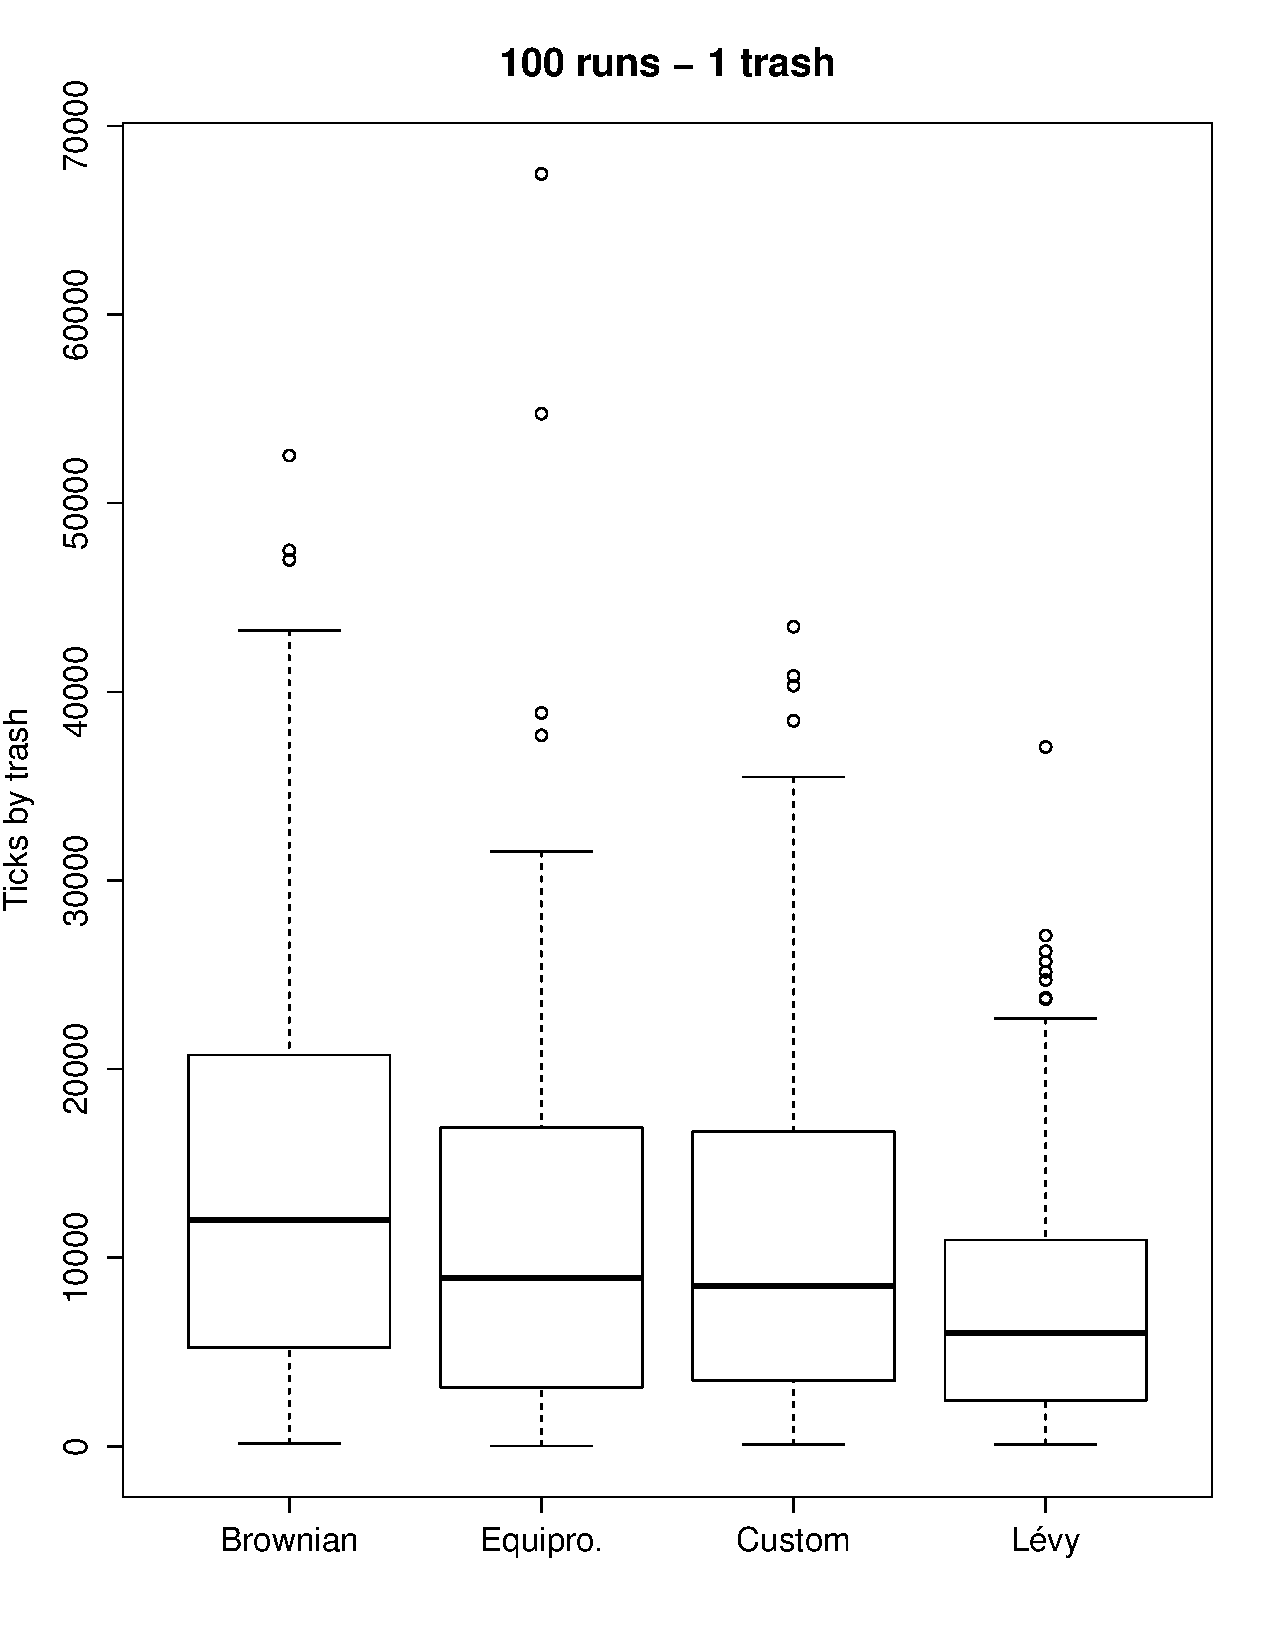
\includegraphics[height=8cm]{diagrams/1Tr_all.pdf}
		\caption{}
		\label{fig:1Trash}
	\end{center}
\end{figure}


Nous avons pour les différentes stratégies les médianes suivantes :

\begin{figure}[H]
	\begin{center}
		\begin{tabular}{ | c | c | }
			\hline
			\multicolumn{2}{ | c | }{Médianes pour 1 débris} \\
			\hline
			Brownian & 11981.75 \\
			Equiprobable & 8939 \\
			Custom & 8494 \\
			Lévy & 5994.25 \\
			\hline
		\end{tabular}
	\end{center}
\end{figure}


Nous pouvons voir que les stratégies Equiprobable et Custom sont
équivalentes lorsqu'il est question de trouver un débris unique.
C'est à dire que leur médiane et leur fiabilité sont équivalentes.

Par contre, nous observons que la stratégie Lévy est deux fois
meilleure que la stratégie Brownian. En effet, sa médiane et sa
fiabilité sont tous deux d'un facteur 2 (ou $\frac{1}{2}$, en fonction du
point de vu).


